%\setRL
%\pagenumbering{arabic} 

\begin{figure}[t]
\begin{center}
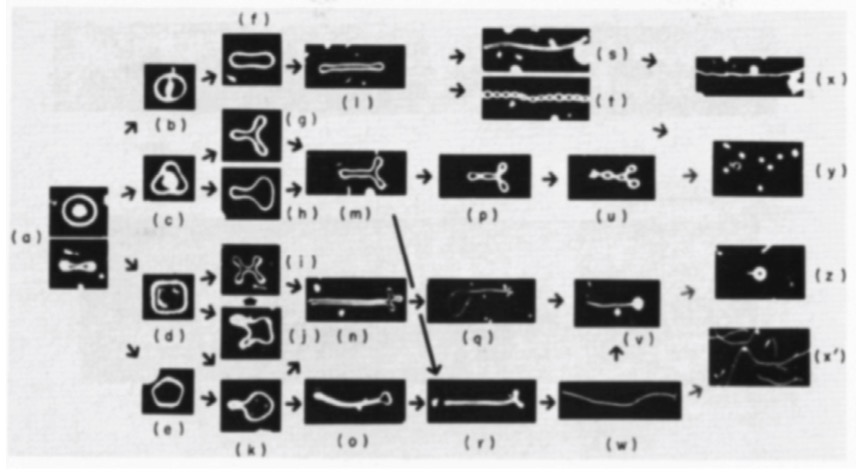
\includegraphics[width=\columnwidth]{\MemBio /Pics/GUVPresChange}
\caption{
مسیر‌های مختلفی که یک غشای غول آسای آب نباتی شکل (ستون سمت چپ، زاویه‌ی دوربین از بالا و کنار) که بر اثر تغییر غلظت نمک محیط طی می‌کند تا به شکل خیلی کشیده (ستون سمت راست) در بیاید.
}
\label{fig:GUVPresChange}
\end{center}
\end{figure}

\begin{figure}[t]
\begin{center}
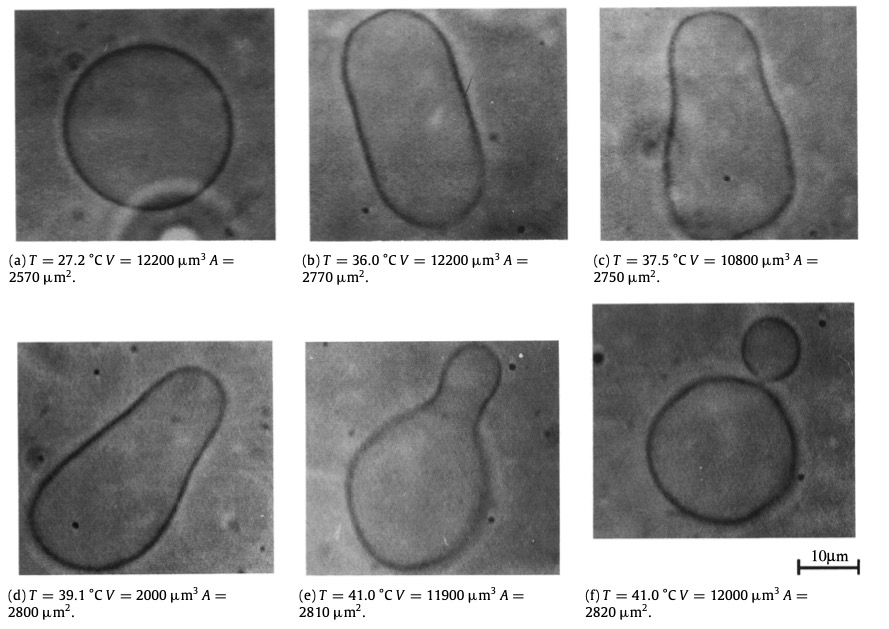
\includegraphics[width=\columnwidth]{\MemBio /Pics/GUVTempChange}
\caption{
تغییر ساختار یک غشای غول ‌آسا به علت تغییر دما از ۲۷/۲ تا ۴۱ درجه‌ی سانتیگراد. در دمای ۳۶ درجه حالت بیضی شکل، بالاتر از دمای ۳۶ شکل گلابی، و با ماندن در دمای ۴۱ درجه یک حباب بر روی آن جدا شده‌است.
}
\label{fig:GUVTempChange}
\end{center}
\end{figure}


محققان با مطالعه‌ی غشا‌های غول‌آسا
\LTRfootnote{Giant Unilamellar vesicle}  
 یا 
 GUV اطلاعات  زیادی راجع به ساماندهی غشاهای چربی جمع‌آوری کرده‌اند. این غشا‌ها را معمولا می‌توان با  مخلوط کردن\LTRfootnote{mixing}  
 غشا‌ و ترکیب‌های چربی در آزمایشگاه ساخت
 \cite{GUVmaking2009}
و اندازه‌ی آن می‌تواند از چند میکرون تا چند میلی‌متر   باشد.
این غشاها از یک دولایه‌ی خیلی ساده لیپیدی تشکیل شده‌اند و در نتیجه‌ ضخامت‌ آن‌ها بین ۴ -۵ میلی‌متر است (دو برابر اندازه‌ی یک مولکول لیپید). غشاهای زیستی ساختار پیچیده‌تری دارند ولی در اصل تمام‌ غشاهای زیستی بر بستر یک ساختار دو لایه‌ی لیپیدی بنا شده‌اند و در نتیجه می‌توان خواص مشترک زیادی میان غشا‌های غول‌آسا و غشاهای زیستی پیدا کرد.
غشاهای دولایه، مرز مشخصی میان شاره‌‌‌ای که درون خود بسته‌بندی کرده‌اند و شاره‌ای که در محیط اطراف است تشکیل می‌دهند. ساختار غشا نسبت به مولکول‌های کوچک غیر باردار مانند 
$H_2O$، 
$O_2$،
و 
$CO_2$
و همچنین
$H_3O^+$
و
$OH^-$
تراوا است ولی نسبت به مولکول‌های درشت‌ترِ حلال در آب مانند گلوکز\LTRfootnote{glucose}
و منوساکارید‌ها\LTRfootnote{monosaccharid}
 تراوا نیست. در نتیجه‌ حضور چنین مولکول‌هایی در محیط، فشار اسمزی بر غشا وارد خواهد کرد. فشار اسمزی به اختلاف غلظت مولکول‌های درون و خارج از غشا بستگی دارد و باعث جابجایی آب داخل غشا می‌شود. در صورتی که غلظت حل شونده در خارج از غشا بیشتر باشد، شبیه به یک پمپ، آب از درون غشا خارج می‌شود و نسبت حجم به سطح غشا را تغییر می‌دهد. برعکس، در صورتی که غلظت مولکول‌ها درون غشا بیشتر از محیط باشد، آب از محیط به درون غشا پمپ می‌شود. تغییر شکل غشا در این صورت تا جایی ادامه پیدا می‌کند که شکل یک کُره به خود بگیرد. اگر همچنان آب به داخل غشا منتقل شود کمی سطح غشا کشیده می‌شود (کُره رشد می‌کند) تا جایی که تحمل کشش غشا تمام شود و غشا پاره خواهد شد.





همانطور که در شکل 
\ref{fig:GUVPresChange}
نشان داده‌ شده‌است، با تغییر غلظت نمک در محیط یک غشایِ لیپیدیِ دارای کلسترول، از شکل اولیه آب نباتیِ\LTRfootnote{biconcave}  
شبیه‌ به گلبول قرمز به حالت کشیده و لوله‌ای در می‌آید. در شکل 
\ref{fig:GUVPresChange}
ساختار‌های هندسی میاینی (و در مواردی ناپایدار) مختلفی که غشا طی می‌کند تا از هندسه‌های سمت چپ به هندسه‌های سمت راست برسد، را می‌توان مشاهده کرد.
GUV نسبت به تغییرات ترمودینامیکی محیط واکنش‌های بسیار جالبی نشان می‌دهد. برای مثال شکل
\ref{fig:GUVTempChange}
ایجاد یک حباب کوچک بر روی یک GUV را با تغییر دمای محیط از ۲۷ تا ۴۱ درجه در قالب ۶ سری عکس پشت سر هم نشان می‌دهد
\cite{MemReviewRamakrishnan2014}.



 

 
 
 
 
 
 
 
 
 
 
 
 